%
%  Vincent Yannello
%
\documentclass[12pt,fullpage]{article}
\usepackage{fullpage}
\usepackage{amsmath}
\DeclareMathOperator{\erf}{erf}
\usepackage{psfrag}                                          % LaTeX graphics tool
\usepackage{pslatex}                                         % avoids the default cmr font
\usepackage{graphicx}                                        % graphics package 
\usepackage{epsfig}                                          % figures
\usepackage{epsfig} 
\usepackage{hyperref}
\usepackage{color}

\begin{document}

\noindent
{\bf Inverted beta distribution} (from \color{blue}\url{http://www.math.wm.edu/~leemis/chart/UDR/UDR.html}\color{black})

\noindent
The shorthand $X \sim {\rm inverted\  beta}(\beta, \gamma)$ is used to indicate that the
random variable $X$ has the inverted beta distribution with parameters $\beta$ and $\gamma$.
A inverted beta random variable $X$ with parameters $\beta$ and $\gamma$ has probability density function 
$$
f(x) = {\frac {{x} ^ {{\it \kern 0.08 em \beta} - 1} \left( x + 1 \right) ^ {- {\it \beta}
 - \gamma}}{B  \left( {\it \beta},\gamma \right) }} \qquad \qquad x > 0,
$$
for $\beta \ge 1$ and $\gamma \ge 1$. 
The probability density function with four different parameter settings is illustrated below.
{\begin{figure}[h!]
\begin{center}
\psfrag{lab1}{$\beta = 1$}
\psfrag{lab2}{$\gamma = 1$}
\psfrag{lab3}{$\gamma = 2$}
\psfrag{lab4}{$\beta = 2$}
\includegraphics[width=3.2in]{InvertedbetaPlot.ps}
\end{center}
\end{figure}}\\
The cumulative distribution, survivor, hazard, cumulative hazard, 
inverse distribution, moment generating, and characteristic functions on the support of $X$ are mathematically intractable.\\ \\
The population mean of $X$ is
$$
E[X] = {\frac {\Gamma  \left( -1+\gamma \right) \Gamma  \left( 1+{\it \beta}
 \right) }{\Gamma  \left( {\it \beta}+\gamma \right) B \left( {\it \beta
},y \right) }}. \qquad \qquad 
$$


\vspace{0.1in}

\newpage
\noindent
{\bf APPL verification:}
The APPL statements
\begin{verbatim}
assume(beta > 1);
assume(y > 1);
X := [[x -> x ^ (beta - 1) * (1 + x) ^ (-beta - y) / Beta(beta, y)],
      [0, infinity],["Continuous", "PDF"]];
Mean(X);
Variance(X);
Skewness(X);
Kurtosis(X);
\end{verbatim}
verify the population mean, variance, skewness, and kurtosis.
\end{document}
